\chapter{Methodology}
\TODO{little bit of an overview of what we're going to achieve in this section}

\section{Grid construction}
\label{sec:method:grid}

A combination of standard and custom OpenFOAM utilities were used to create three grids: BTF, SLEVE, and a cut cell style grid.  OpenFOAM grids comprise a set of cells connected by shared faces.  A face is composed from a list of points that form the face vertices.
OpenFOAM uses a three dimensional cartesian coordinate system.  Since all tests presented here are two dimensional $x-z$ plane, empty boundary conditions are used on the front and back faces to ensure that no solutions are required in the $y$ direction.

Two dimensional, regular cartesian grids were created using the OpenFOAM utility, \shellcmd{blockMesh}.  A custom utility was used to modify these orthogonal grids by adjusting the height of points to create terrain following grids.

Most implementations of terrain following layers use a coordinate system that makes the domain rectangular, but introduces metric terms into the equations of motion (more detail was presented in section~\ref{sec:theory:coord-transform}).  Instead, the model presented here uses cartesian coordinates and unstructured grids.  By doing so, results from the same model can be compared between terrain following and cut cell grids without modifying the equation set or discretisation.

\begin{figure}
	\centerfloat
	\includegraphics[height=2.8in,angle=270]{mesh-snapCol-schaerExp-resting.eps}
	\caption{A `SnapCol' grid, \SI{20}{\kilo\meter} wide and \SI{2}{\kilo\meter} high, created by intersecting the terrain surface with a regular grid as described in section~\ref{sec:method:grid}.  Note that, unlike a true cut cell grid, some small cells have faces at $z = \SI{500}{\meter}$ that are not entirely horizontal.}
	\label{fig:method:cut-cell}
\end{figure}

At the time of writing, OpenFOAM does not directly support cut cell grids\footnote{An enhancement request was filed in 2013 to add support for cartesian cut cells to OpenFOAM, see \url{http://www.openfoam.org/mantisbt/view.php?id=1083}}.  Instead, the \shellcmd{snappyHexMesh} OpenFOAM utility was used to create a grid that approximates the cut cell method.  First, a custom utility was used to move points beneath the surface up to the surface creating small cells near mountain peaks.  Second, a description of the surface was taken from any of the terrain following grids and \shellcmd{snappyHexMesh} was used to intersect the surface with the grid.  The tool removes cells whose centres are below the surface.  An example of the resulting grid is shown in figure~\ref{fig:method:cut-cell}.

The grid is not strictly a cut cell mesh because, when \shellcmd{snappyHexMesh} moves points along the surface according to its heuristics, some points are moved horizontally.  It has not been possible to correct this issue for this project.  This grid is referred to as the `SnapCol' grid throughout this project.


\section{Discretisation of Euler equations}
\label{sec:method:discretisation}

\TODO{need to explain Lorentz staggering because we'll talk about its computational mode in gravityWaves results}

The fully-compressible Euler equations used in the resting atmosphere test (section~\ref{sec:resting}) and gravity waves test (section~\ref{sec:gw}) are specified as
\begin{align}
	& \text{Momentum} & \frac{\partial \rho \vect{u}}{\partial t} + \del \cdot \rho \vect{u} \vect{u} &= \rho \vect{g} - c_p \rho \theta \del \exner \label{eqn:method:momentum} \\
%
& \text{Continuity} & \frac{\partial \rho}{\partial t} + \del \cdot \rho \vect{u} &= 0 \label{eqn:method:continuity} \\
%
& \text{Potential temperature (flux form)} & \frac{\partial \rho \theta}{\partial t} + \del \cdot \rho \vect{u} \theta &= 0 \\
%
& \text{Potential temperature (advective form)} & \frac{\partial \theta}{\partial t} + \vect{u} \cdot \del \theta &= 0 \\
%
& \text{Equation of state} & \exner^{(1 - \kappa / \kappa)} &= \frac{R \rho \theta}{p_0}
\end{align}
where $\rho$ is the density, $\vect{u}$ is the velocity field, $\vect{g}$ is gravitational acceleration, $c_p$ is the heat capacity of dry air at constant pressure, $\theta$ is the potential temperature, $\exner = \left( p / p_0 \right)^\kappa$ is the Exner function of pressure, $p$ is the pressure, $p_0$ is a reference pressure, $\kappa = R/c_p$, and $R$ is the specific gas constant of dry air.

Here, we outline the placement of prognostic variables, pressure gradient discretisation, and the advection scheme.  Further details of the discretisation are given by \textcite{weller-shahrokhi2014}.

\begin{figure}
	\captionsetup[subfigure]{position=b}
	\centering
	\subcaptionbox{Vertical cross section of geometry}[0.48\textwidth]{\documentclass[tikz]{standalone}
\usepackage{bm}
\newcommand{\vect}{\bm}
\newcommand{\del}{\nabla}

\begin{document}
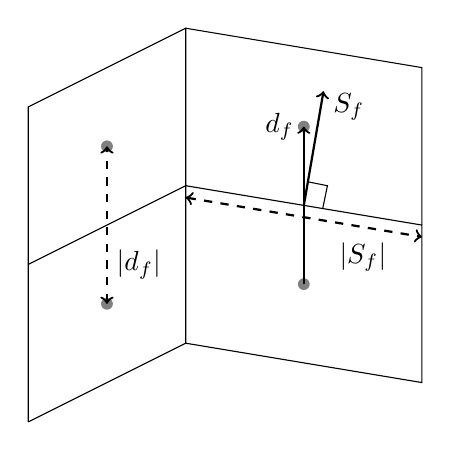
\begin{tikzpicture}[
  scale=0.5,
  cpnt/.style={fill=gray},
  arr/.style={thick, ->},
  mag/.style={dashed, thick, <->}
]
\draw (0,0) --  (4,2)  -- (4,6)  -- (0,4) -- (0,0);
\draw (4,2) --  (10,1) -- (10,5) -- (4,6);
\draw (0,4) --  (0,8)  -- (4,10)  -- (4,6);
\draw (10,5) -- (10,9) -- (4,10);
\path [cpnt] (2,3) circle [radius=0.15];
\path [cpnt] (2,7) circle [radius=0.15];
\path [cpnt] (7,3.5) circle [radius=0.15];
\path [cpnt] (7,7.5) circle [radius=0.15];
\draw [arr] (7,3.5) -- (7,7.5);
\draw [arr] (7,5.5) -- (7.5,8.4);
\node [left] at (7,7.5) {$\vect{d}_f$};
\node [right] at (7.5,8) {$\vect{S}_f$};
\draw [mag] (2,3) -- (2,7);
\node [right] at (2,4) {$|{\vect{d}_f}|$};
\draw [mag] (4,5.7) -- (10,4.7);
\node [below] at (8.5,4.8) {$|{\vect{S}_f}|$};
\draw (7.48,5.42) -- (7.6,6) -- (7.1,6.1);
\end{tikzpicture}
\end{document}
}
	\hfill
	\subcaptionbox{Placement of prognostic variables}[0.48\textwidth]{\documentclass[tikz]{standalone}
\usepackage{bm}
\newcommand{\vect}{\bm}
\newcommand{\del}{\nabla}

\newcommand{\trans}[1]{{#1^\star}}
\newcommand{\surface}{h}
\newcommand{\shellcmd}[1]{\texttt{#1}}
\newcommand{\diffusioncoeff}{\mathcal{D}}
\newcommand{\exner}{\Pi}
\newcommand{\courant}{\mathrm{Co}}

\begin{document}
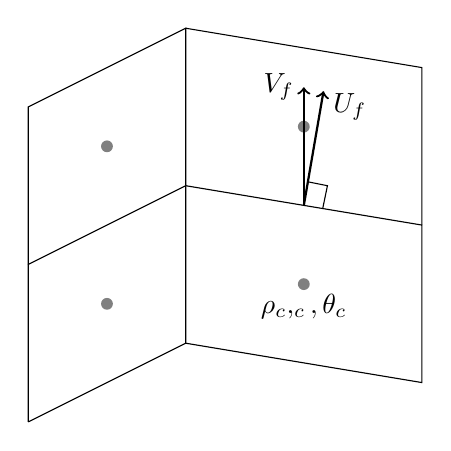
\begin{tikzpicture}[
  scale=0.5,
  cpnt/.style={fill=gray},
  arr/.style={thick, ->},
  mag/.style={dashed, thick, <->}
]
\draw (0,0) --  (4,2)  -- (4,6)  -- (0,4) -- (0,0);
\draw (4,2) --  (10,1) -- (10,5) -- (4,6);
\draw (0,4) --  (0,8)  -- (4,10)  -- (4,6);
\draw (10,5) -- (10,9) -- (4,10);
\path [cpnt] (2,3) circle [radius=0.15];
\path [cpnt] (2,7) circle [radius=0.15];
\path [cpnt] (7,3.5) circle [radius=0.15];
\path [cpnt] (7,7.5) circle [radius=0.15];
\draw [arr] (7,5.5) -- (7,8.5);
\draw [arr] (7,5.5) -- (7.5,8.4);
\node [below] at (7,3.5) {$\rho_c, \exner_c, \theta_c$};
\node [left] at (7,8.5) {$V_f$};
\node [right] at (7.5,8) {$U_f$};
\draw (7.48,5.42) -- (7.6,6) -- (7.1,6.1);
\end{tikzpicture}
\end{document}
}
	\caption{Geometric placement of prognostic variables in two dimensions.  Adapted from \textcite{weller-shahrokhi2014}.}
	\label{fig:method:placement}
\end{figure}

To solve the continuity equation (equation~\ref{eqn:method:continuity}), in section~\ref{sec:theory:fv} we found that we must calculate the flux across all cell faces (see equation~\ref{eqn:theory:discrete-continuity}).  To do this, we first find the mass flux component $V_f$ in the direction between cell centres such that
\begin{align}
	V_f &= \rho \vect{u} \cdot \vect{d}_f
%
\intertext{where $\vect{d}_f$ is the vector between the centres of the two cells who share the face $f$.  Second, we use the H operator given in \textcite{weller-shahrokhi2014} to find the mass flux normal to the surface, $U_f$, that is}
%
	U &= HV
\end{align}
where $U_f = \rho \vect{u} \cdot \vect{S}_f$, and $\vect{S}_f$ is normal to the face $f$ having a magnitude equal to the face area.  \textcite{thuburn-cotter2012} recommend the use of $V$ instead of $U$ as the prognostic variable to obtain mimetic properties including a curl-free pressure gradient.  The geometry just described is summarised in figure~\ref{fig:method:placement}.

The Exner gradient at a face $f$ in the direction between cell centres, $\del_d \exner$, is calculated from the exner value of the two cells who share the face \autocite{weller-shahrokhi2014}
\begin{align}
	\del_d \exner = \frac{1}{| \vect{d}_f |} \sum_{c \in\: f} - n_f \exner_c
%
\intertext{where $n_f$ corrects for the face orientation so that}
%
	n_f =
	\begin{cases}
		1  & \text{if $\vect{S}_f$ points away from the cell} \\
		-1 & \text{if $\vect{S}_f$ points toward the cell}
	\end{cases}
\end{align}

\begin{figure}
	\centering
	\documentclass[tikz]{standalone}
\usepackage{bm}
\newcommand{\vect}{\bm}
\newcommand{\del}{\nabla}

\newcommand{\trans}[1]{{#1^\star}}
\newcommand{\surface}{h}
\newcommand{\shellcmd}[1]{\texttt{#1}}
\newcommand{\diffusioncoeff}{\mathcal{D}}
\newcommand{\exner}{\Pi}
\newcommand{\courant}{\mathrm{Co}}

\begin{document}
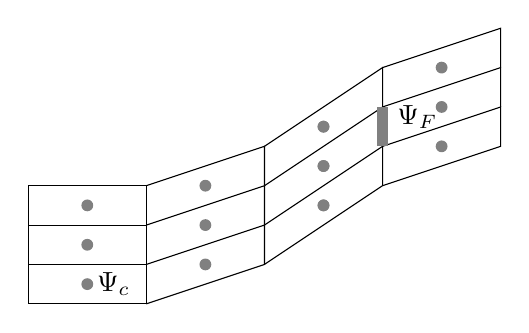
\begin{tikzpicture}[
  scale=0.5,
  cpnt/.style={fill=gray},
]
\draw (0,0) -- (3,0) -- (3,1) -- (0,1) -- (0,0);
\draw (0,1) -- (3,1) -- (3,2) -- (0,2) -- (0,1);
\draw (0,2) -- (3,2) -- (3,3) -- (0,3) -- (0,2);

\draw (3,0) -- (6,1) -- (6,2) -- (3,1);
\draw (6,2) -- (6,3) -- (3,2);
\draw (6,3) -- (6,4) -- (3,3);

\draw (6,1) -- (9,3) -- (9,4) -- (6,2);
\draw (9,4) -- (9,5) -- (6,3);
\draw (9,5) -- (9,6) -- (6,4);

\draw (9,3) -- (12,4) -- (12,5) -- (9,4);
\draw (12,5) -- (12,6) -- (9,5);
\draw (12,6) -- (12,7) -- (9,6);

\draw[line width=4, gray] (9,4) -- (9,5) node [pos=0.75,right,black] {$\Psi_F$};

\path [cpnt] (1.5,0.5) circle [radius=0.15] node [right] {$\Psi_c$};
\path [cpnt] (1.5,1.5) circle [radius=0.15];
\path [cpnt] (1.5,2.5) circle [radius=0.15];

\path [cpnt] (4.5,1) circle [radius=0.15];
\path [cpnt] (4.5,2) circle [radius=0.15];
\path [cpnt] (4.5,3) circle [radius=0.15];

\path [cpnt] (7.5,2.5) circle [radius=0.15];
\path [cpnt] (7.5,3.5) circle [radius=0.15];
\path [cpnt] (7.5,4.5) circle [radius=0.15];

\path [cpnt] (7.5,2.5) circle [radius=0.15];
\path [cpnt] (7.5,3.5) circle [radius=0.15];
\path [cpnt] (7.5,4.5) circle [radius=0.15];

\path [cpnt] (10.5,4) circle [radius=0.15];
\path [cpnt] (10.5,5) circle [radius=0.15];
\path [cpnt] (10.5,6) circle [radius=0.15];

\end{tikzpicture}
\end{document}

	\caption{Two-dimensional cubic upwind stencil used in advecting momentum and potential temperature.  A face value $\Psi_F$ is interpolated from cell values, $\Psi_c$, denoted by grey dots.  Adapted from \textcite{weller-shahrokhi2014}.}
	\label{fig:method:cubicUpwind}
\end{figure}

Momentum and potential temperature are advected using an upwind-biased cubic interpolation.  A multi-dimensional cubic function is used whose coefficients are found using a least-squares fit with cell data in the stencil.  These coefficients are used to weight the cell values within the stencil, and the weighted sum is used to calculate $\Psi_F$.  A two-dimensional stencil is shown in figure~\ref{fig:method:cubicUpwind}.

\section{Energy measures}
\label{sec:method:energy}

Energy conservation is desirable in the discretisation of the Euler equations.  In the resting atmosphere test detailed in section~\ref{sec:resting}, energy is conserved in the analytic solution, but not in all numerical approximations.  The normalised energy change $\Delta E$ at time $t$ is found by comparing with the initial energy measure, hence
\begin{align}
	\Delta E(t) &= \frac{E(t) - E(t = \SI{0}{\second})}{E(t = \SI{0}{\second})}
\end{align}
Three energy measures are considered, where the volume integral of some field $\varphi$ is the volume-weighted sum given by
\begin{align}
	\int_V \varphi \diff{V} &= \frac{\sum_c \varphi_c V_c}{\sum_c V_c}
\end{align}
First, kinetic energy $E_K$ is calculated as \autocite{thuburn2014}
\begin{align}
	E_K(t) &= \int_V \frac{1}{4} \sum_{f \in \: c} \frac{\vect{u} \cdot \vect{S}_f \: \vect{u} \cdot \vect{d}_f}{V_c} \diff{V}
%
	\intertext{Second, potential energy $E_P$ is}
%
	E_P(t) &= - \int_V \rho \vect{g} \cdot \vect{x}_c \diff{V}
%
	\intertext{where $\vect{x}_c$ is the position vector of the centre of cell $c$.  Third, the internal energy $E_I$ is \TODOcite}
%
	E_I(t) &= \int_V \rho \theta \Pi c_v \diff{V}
\end{align}
where $c_v$ is the heat capacity of dry air at constant volume.

\section{Courant--Friedrichs--Lewy criterion}
The Courant--Friedrichs--Lewy (CFL) criterion is a necessary condition for numerical stability (though it is not always, by itself, a sufficient condition).  For an explicit advection scheme, it constrains the timestep as a function of wind speed and cell volume.  This is especially relevant for the small cells produced by the piecewise linear shaving technique described in section~\ref{sec:theory:shaving}.

The CFL criterion states that the numerical domain of dependence must contain the true domain of dependence for the scheme to be convergent \autocite{leveque2002}.  \TODO{present a small 1D example with diagram, arrive at 1D courant number}.

On a two-dimensional unstructured grid, the Courant number for cell $c$ is \autocite{weller-shahrokhi2014}
\begin{align}
	\courant_c = \frac{\Delta t}{2 V_c} \sum_{f \in\: c} \vect{u} \cdot \vect{S}_f
\end{align}
so that the CFL criterion is $\courant_c < 1 \forall c$.

